\documentclass[12pt,a4paper,oneside]{article}

\usepackage[utf8]{inputenc}
\usepackage[russian,english]{babel}
\usepackage[T2A]{fontenc}

\usepackage{hyperref}
\usepackage[final]{listings}
\usepackage{breakurl}
\usepackage{cite}
\usepackage{perpage}

\usepackage[dvips]{graphicx}
\graphicspath{{img/}}

\def\UrlBreaks{\do\/\do-}

\lstset{
  frame=single,
  breaklines=true,
  basicstyle=\small,
  postbreak=\raisebox{0ex}{\ensuremath{\hookrightarrow\space}},
  numbers=left
}

\renewcommand{\thefigure}{\thesection.\arabic{figure}}
\MakePerPage{footnote}

\title{Домашнее задание 2. \\ Аллокация памяти.}
\author{Я}
\date{\today}

\begin{document}
  \sloppy
  \maketitle
  \tableofcontents
  \clearpage

  \section{Основное задание}

Это домашнее задание является вводным, в нем вам необходимо настроить
последовательный порт, контроллер прерываний и интервальный таймер.

\begin{enumerate}
  \item Инициализировать контроллер последовательного порта и создать функцию
        записи в последовательный порт. Мы будем использовать последовательный
        порт вместо экрана.
  \item Настроить прогораммируемый контроллер прерываний i8259~\cite{INTEL:8259}
        (такой раньше использовался в персональных компьютерах, но сейчас его не
        используют, ему на замену пришел APIC, который поддерживает обратную
        совместимость).
  \item Настроить программируемый интервальный таймер~\cite{INTEL:8253} на
        прерывания через равные интервалы времени. В обработчике прерывания вам
        нужно выводить на последотвальный порт сообщение (текст сообщения не
        существеннен, но перед тем как расходиться, помните, что у проверяющего
        может отсутствовать чувство юмора и шутка может плохо закончится).
\end{enumerate}

\section{Дополнительные задания}

\begin{itemize}
  \item В целях отладки очень часто полезно видеть backtrace, т. е. как
        программа пришла к той или иной строчке кода. Задание заключается в том
        чтобы написать функцию, которая выводит backtrace в последовательный
        порт в виде набора аддресов. Используйте эту функцию в обработчике
        исключений. При этом запрещается инструментировать функции, т. е.
        нельзя модифицировать функции, чтобы они самостоятельно добавляли себя
        в backtrace.
  \item Реализуйте функции семейства *printf (а именно printf, vprintf,
        snprintf и vsnprintf). Функция должна поддерживать как минимум
        следующие спецификаторы формата: d, i, u, o, x, c, s, p, и следующие
        модификаторы размера: hh, h, l, ll, z~\cite{CPP:PRINTF}. При реализации
        нельзя ограничивать размер вывода одного вызова printf/vprintf каким-то
        фиксированным размером, т. е. нельзя просто реализваоть \{v\}snprintf и
        вызвать ее из \{v\}printf передав буффер фиксированного размера. 
\end{itemize}

  \begin{frame}
\frametitle{Paging}

\begin{itemize}
  \item отображение VA на PA с гранулярностью в Page (блок память фиксированного размера);
  \item привилегии/права доступа проверяются на уровне страниц - меньше гранулярность;
  \item отображение описывается иерархической структурой (Page Table, далее PT) - большая гибкость;
  \item каждый процесс имеет свою PT - процессы изолированы друг от друга;
\end{itemize}
\end{frame}

\begin{frame}
\frametitle{Paging}
\framesubtitle{Таблицы страниц}

\begin{figure}
  \centering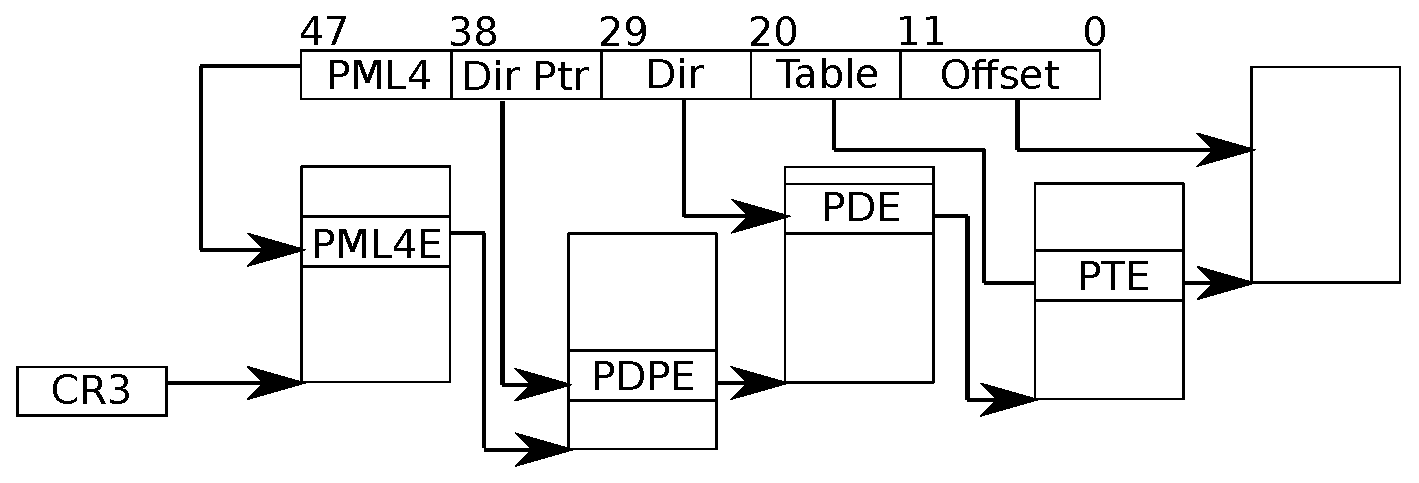
\includegraphics[width=.9\linewidth]{arch-page}
  \caption{x86-64 Page Tables}
\end{figure}
\end{frame}

\begin{frame}
\frametitle{Paging}
\framesubtitle{Права доступа и прочее}

\begin{itemize}
  \item Paging позволяет защитить память от доступа непривилегированного кода;
  \item Paging позволяет защитить память от доступа привилегированного кода (SMEP/SMAP - защита kernelspace от атак из userspace);
  \item Paging позволяет запрещать исполнение кода в участке памяти;
  \item Paging позволяет управлять кешированием участка памяти;
  \item Paging вытеснил сегментацию (сегментация все еще используется в очень специфичных случаях);
\end{itemize}
\end{frame}

\begin{frame}
\frametitle{Paging}
\framesubtitle{Translation Lookaside Buffer}

\begin{itemize}
  \item<1-> Обращение к PT при каждом доступе к памяти - очень дорого
    \begin{itemize}
      \item чем больше памяти - тем больше уровней
      \item чем больше уровней - тем дороже трансляция
      \item чем больше памяти - тем меленее работа с ней (короче, все плохо)
    \end{itemize}
  \item<2-> Кеширование ускоряет процесс, но задача слишком специфичная - используем специальный кеш TLB;
  \item<3-> TLB не прозрачен для программиста - при изменении в PT нужно явно сбросить TLB;
\end{itemize}
\end{frame}

\begin{frame}
\frametitle{Page Fault}

Page Fault происходит если:
\begin{itemize}
  \item для виртуального адреса отсутствует отображение в физический (в x86 за это отвечает бит Present);
  \item отображение есть, но не достаточно прав доступа для обращения к памяти;
  \item произошла попытка записи в страницу только для чтения;
  \item произошла попытка исполнить кода со страницы не предназначенной для исполнения;
  \item обнаружена запись некорректного формата в PT;
\end{itemize}

\onslide<2->{Fault (в терминологии x86) - ошибка, которую можно исправить, виртуальный адрес по которому происходит обращение прилагается.}

\end{frame}

\begin{frame}
\frametitle{Page Fault}
\framesubtitle{On Demand Allocation}

\begin{figure}
  \centering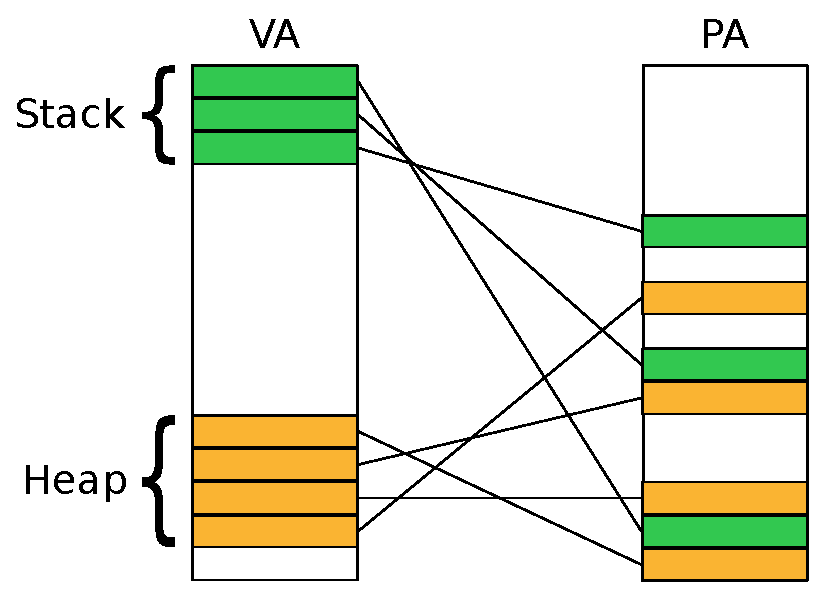
\includegraphics[width=.8\linewidth]{page-demand0}
  \caption{Отображение VA на PA}
\end{figure}
\end{frame}

\begin{frame}
\frametitle{Page Fault}
\framesubtitle{On Demand Allocation}

\begin{figure}
  \centering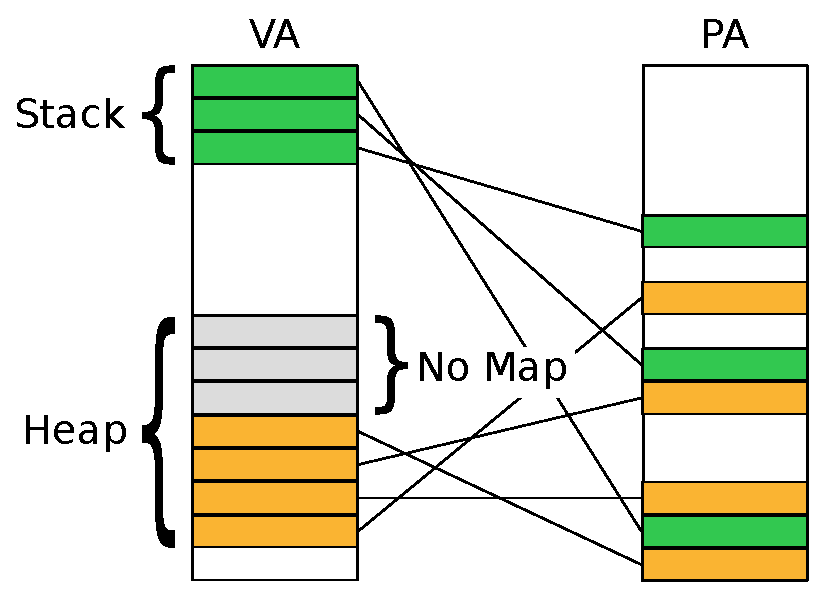
\includegraphics[width=.8\linewidth]{page-demand1}
  \caption{Процесс увеличивает Heap - страницы не выделяются}
\end{figure}
\end{frame}

\begin{frame}
\frametitle{Page Fault}
\framesubtitle{On Demand Allocation}

\begin{figure}
  \centering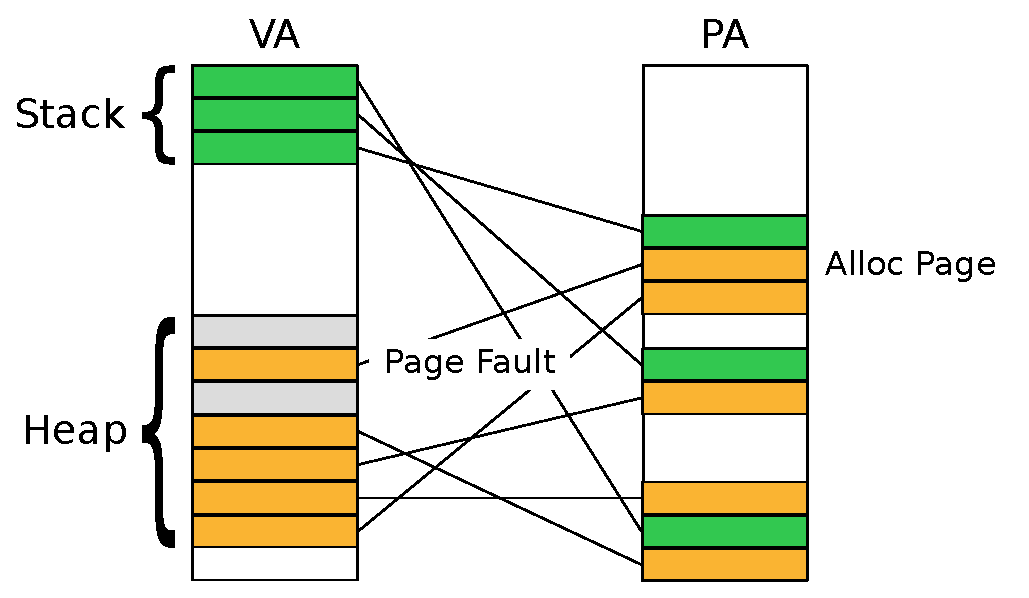
\includegraphics[width=.9\linewidth]{page-demand2}
  \caption{При обращении происходит Page Fault - выделяем страницу}
\end{figure}
\end{frame}

\begin{frame}
\frametitle{Page Fault}
\framesubtitle{On Demand Allocation}

\begin{itemize}
  \item<1-> аллоцируются только страницы, к котором происходит обращение - если процесс не использует память аллоцировать ее тоже не нужно;
  \item<2-> если ОС сказала, что аллоцировала память, еще не значит что она правда ее аллоцировала; \onslide<3->{с этим можно частично бороться:
    \begin{itemize}
      \item держать запас физических страниц для Page Fault;
      \item swapping может предотвратить самое худшее;
    \end{itemize}}
\end{itemize}
\end{frame}

\begin{frame}
\frametitle{Fork}
\framesubtitle{Копирование VA}

fork - системный вызов в Unix-like системах для создания нового процесса. Новый
процесс является копией старого. Т. е. нужно копировать VA:

\begin{itemize}
  \item честная копия VA может привести к большому количеству аллокаций физической памяти;
  \item честная копия VA может потребовать копирования большого количества памяти;
  \item<2-> честная копия, на самом деле, не нужна:
    \begin{itemize}
       \item не нужно копировать Read Only части VA;
       \item не нужно копировать то, что мы не будем использовать;
    \end{itemize}
\end{itemize}
\end{frame}

\begin{frame}
\frametitle{Page Fault}
\framesubtitle{Copy On Write}

\begin{figure}
  \centering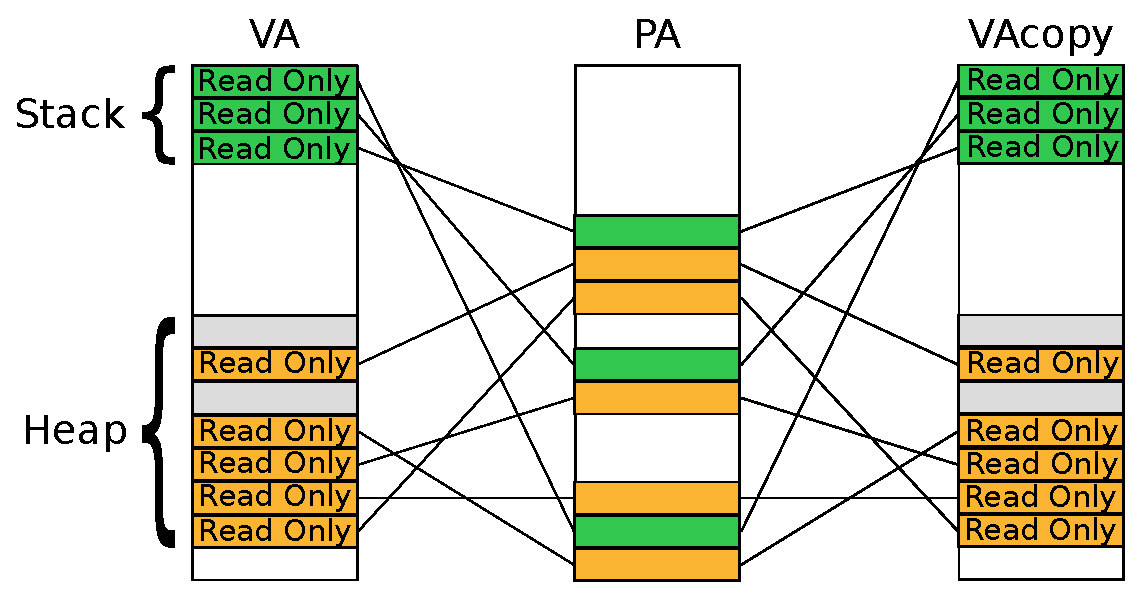
\includegraphics[width=.9\linewidth]{page-cow0}
  \caption{При копировании VA и оригинал и копия используют права Read Only}
\end{figure}
\end{frame}

\begin{frame}
\frametitle{Page Fault}
\framesubtitle{Copy On Write}

\begin{figure}
  \centering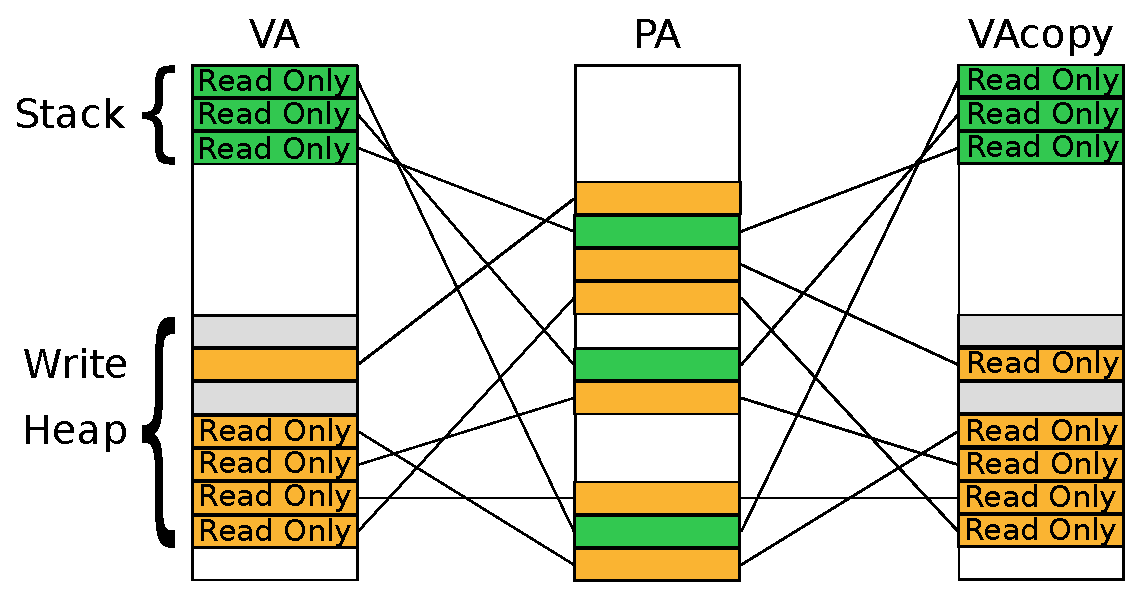
\includegraphics[width=.9\linewidth]{page-cow1}
  \caption{При записи происходит аллокация и настоящее копирование}
\end{figure}
\end{frame}

\begin{frame}
\frametitle{Page Fault}
\framesubtitle{Copy On Write}

\begin{figure}
  \centering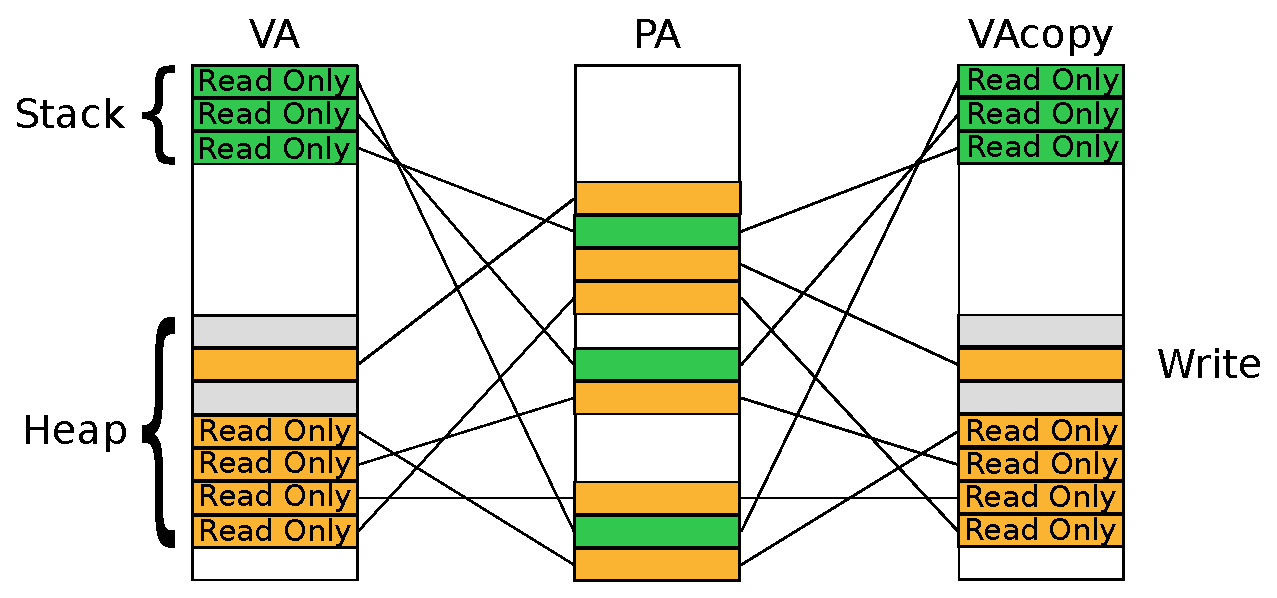
\includegraphics[width=.9\linewidth]{page-cow2}
  \caption{При записи происходит аллокация и настоящее копирование}
\end{figure}
\end{frame}

\begin{frame}
\frametitle{Page Fault}
\framesubtitle{Copy On Write}

\begin{figure}
  \centering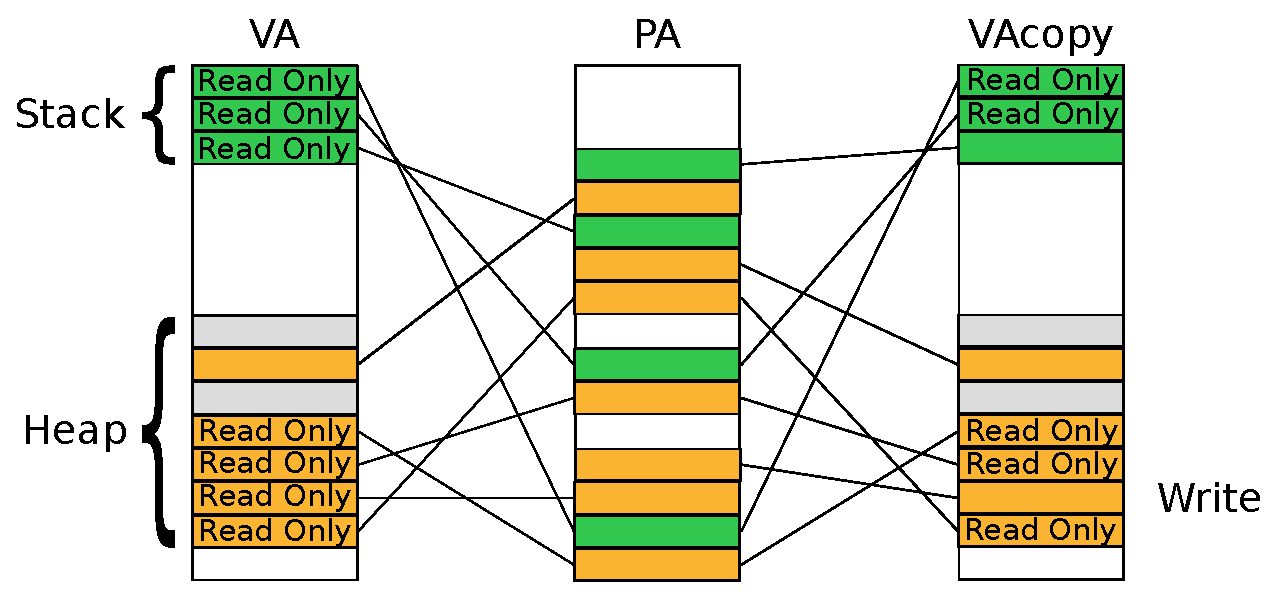
\includegraphics[width=.9\linewidth]{page-cow3}
  \caption{При записи происходит аллокация и настоящее копирование}
\end{figure}
\end{frame}

\begin{frame}
\frametitle{Page Fault}
\framesubtitle{Copy On Write}

\begin{figure}
  \centering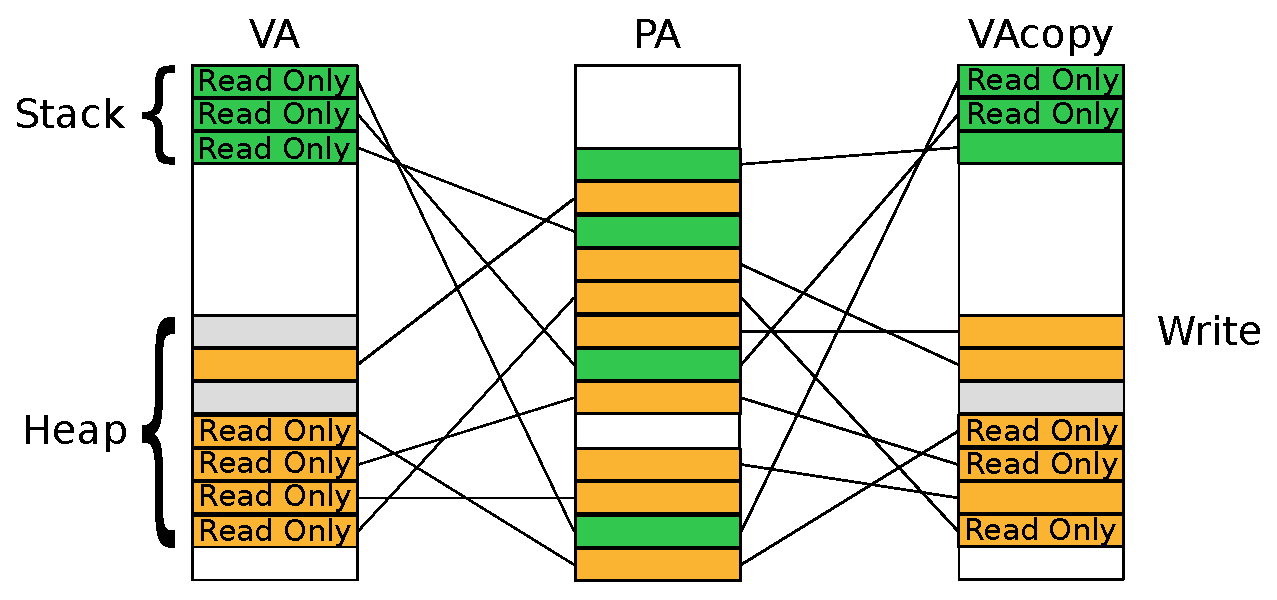
\includegraphics[width=.9\linewidth]{page-cow4}
  \caption{При записи происходит аллокация и настоящее копирование}
\end{figure}
\end{frame}

\begin{frame}
\frametitle{Page Fault}
\framesubtitle{Copy On Write}

Для реализации Copy On Write, кроме наличия Page Fault, еще необходимы:
\begin{itemize}
  \item счетчик ссылок для физических страниц - мы должны знать, что страницу нужно копировать;
    \begin{itemize}
      \item если вы используете Buddy Allocator, то у вас уже есть дескриторы для страниц - в них можно хранить счетчик ссылок;
    \end{itemize}
  \item "предполагаемые" права доступа к странице - мы должны знать, правда ли страница Read Only, или только из-за Copy On Write.
    \begin{itemize}
      \item для каждого процесса должна быть структура описывающая его VA (в Linux Kernel она называется mm\_struct, в FreeBSD она называется vmspace, в MAC OS X она называется vm\_map)
    \end{itemize}
\end{itemize}
\end{frame}

\begin{frame}
\frametitle{Non-Contigous Page Allocation}

\begin{itemize}
  \item<1-> Аллокация больших блоков памяти может провалиться из-за фрагментации.
  \item<2-> Paging позволяет отобразить последовательные участки VA на непоследовательные участки PA.
  \item<3-> Необходимо только иметь участок VA достаточного размера.
\end{itemize}
\end{frame}

\begin{frame}
\frametitle{Адресное пространство процесса}

\begin{columns}[T]
  \begin{column}{.4\textwidth}
    \begin{figure}
      \centering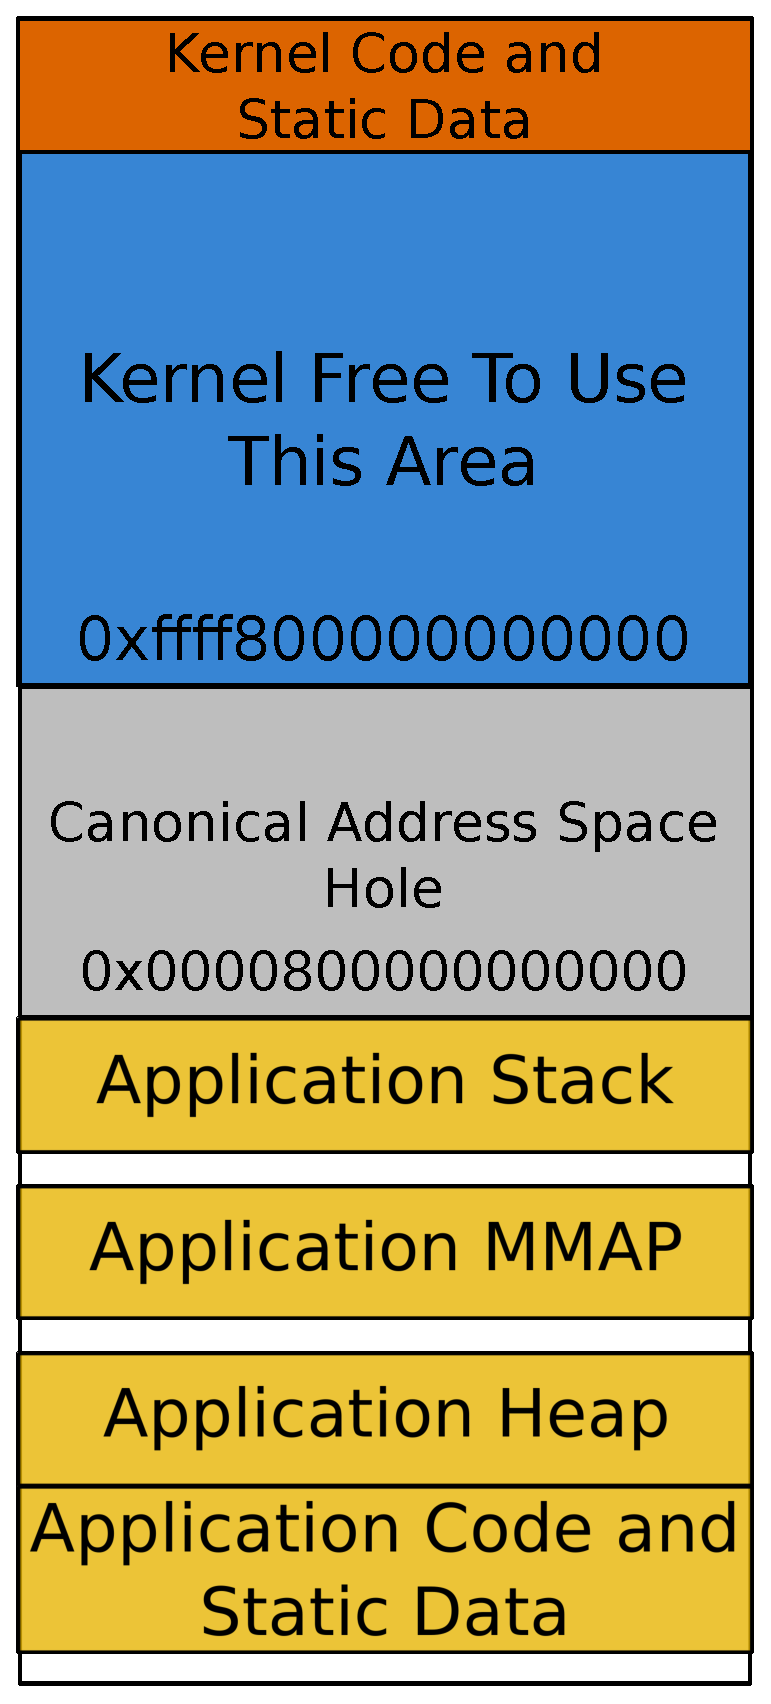
\includegraphics[height=.6\textheight]{memmap}
      \caption{Типичная структура VA на x86-64}
    \end{figure}
  \end{column}
  \begin{column}{.5\textwidth}
    \begin{itemize}
      \item Процессоры Intel поддерживают порядка 2TB RAM.
      \item У нас есть $2^{47} - 2GB$ VA между "дырой" и ядром (по факту, бесконечное VA).
      \item Будем аллоцировать непрерывные участки VA и отображать страницы на них.
    \end{itemize}
  \end{column}
\end{columns}
\end{frame}

\begin{frame}
\frametitle{There is much more about paging}

За кадром осталось много полезных тем:
\begin{itemize}
  \item<2-> использование свободных страниц (коснемся этого когда дойдем до ФС)
    \begin{itemize}
      \item свободная память - бесполезная память;
      \item Page Cache, Buffer Cache, и много других;
    \end{itemize}
  \item<3-> swapping:
    \begin{itemize}
      \item swapping возможен и без Paging-а;
      \item Paging позволяет не выгружать все VA процесса на диск;
    \end{itemize}
  \item<4-> для Linux Kernel есть подробное (немного устаревшее) описание по \href{https://www.kernel.org/doc/gorman/}{ссылке}
\end{itemize}

\end{frame}

  \begin{frame}
\frametitle{Классы памяти}

\onslide<1->{По привелегиям доступа:
\begin{enumerate}
  \item привелигерованная (kernel space)
  \item не привелигерованная (user space)
\end{enumerate}}

\onslide<2->{По способу аллокации:
\begin{enumerate}
  \item статическая память (код, глобальные перменные - размер известен заранее)
  \item динамическая память (куча, free store и тд - размер не известен заранее)
\end{enumerate}}
\end{frame}

\begin{frame}
\frametitle{Карта памяти}

\begin{columns}[T]

  \begin{column}{.4\textwidth}
    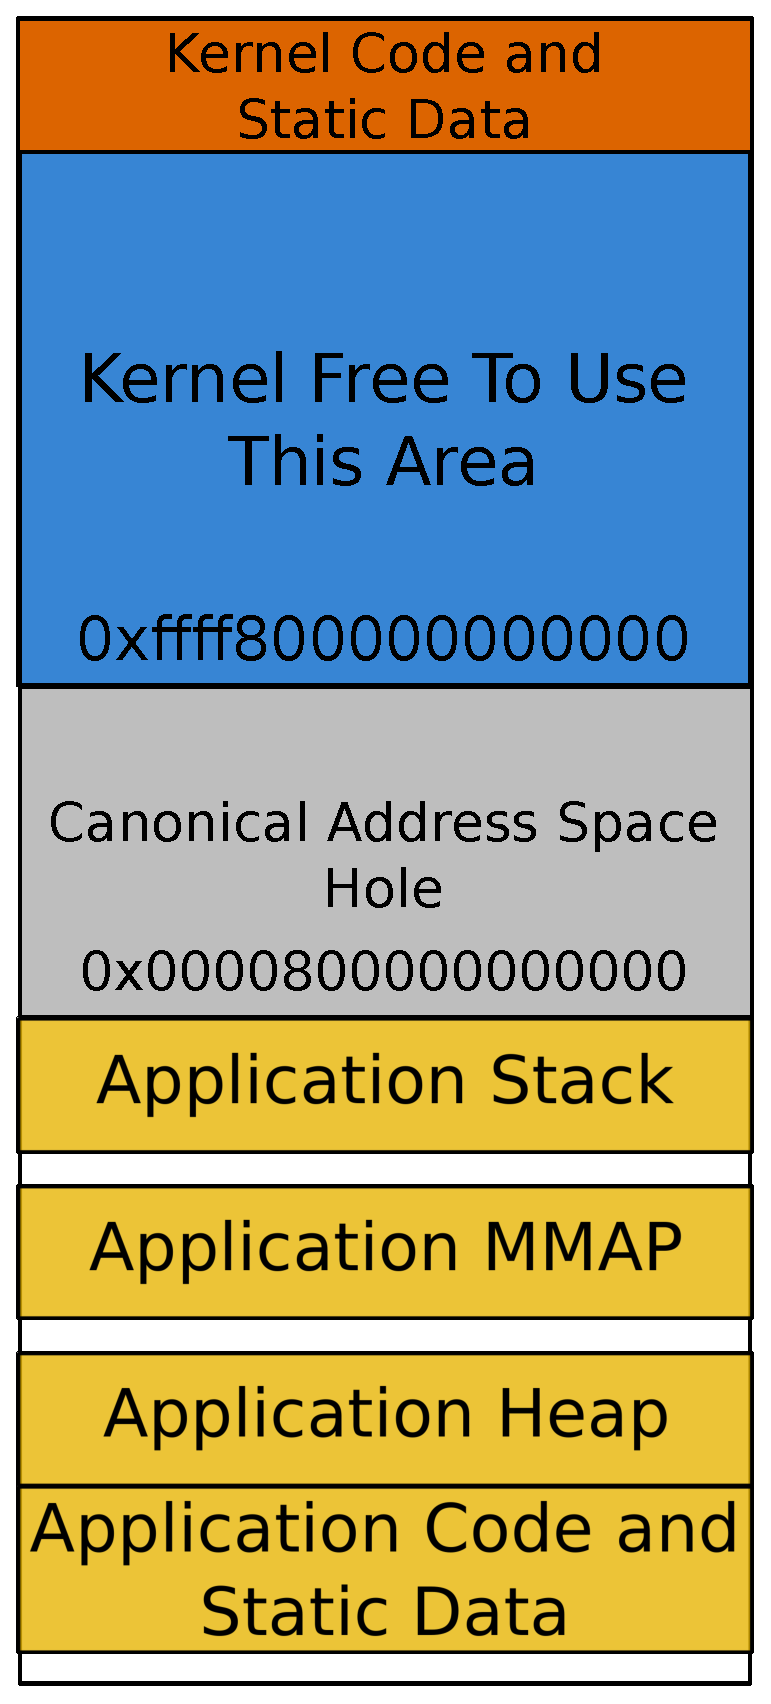
\includegraphics[width=.8\linewidth]{memmap}
  \end{column}

  \begin{column}{.6\textwidth}
    \begin{itemize}
      \item Kernel Code and Static Data - привелигерованная статическая память (System V ABI amd64, 3.5.1 Architectural Constraints, Kernel code model)
      \item Canonical Address Space Hole - недопустимые адреса памяти (Intel\textsuperscript{\textregistered} 64 and IA-32 Architectures Software Developer's Manual, 3.3.7.1 Canonical Addressing)
    \end{itemize}
  \end{column}
\end{columns}

\end{frame}

\begin{frame}
\frametitle{Карта памяти}

\begin{columns}[T]

  \begin{column}{.4\textwidth}
    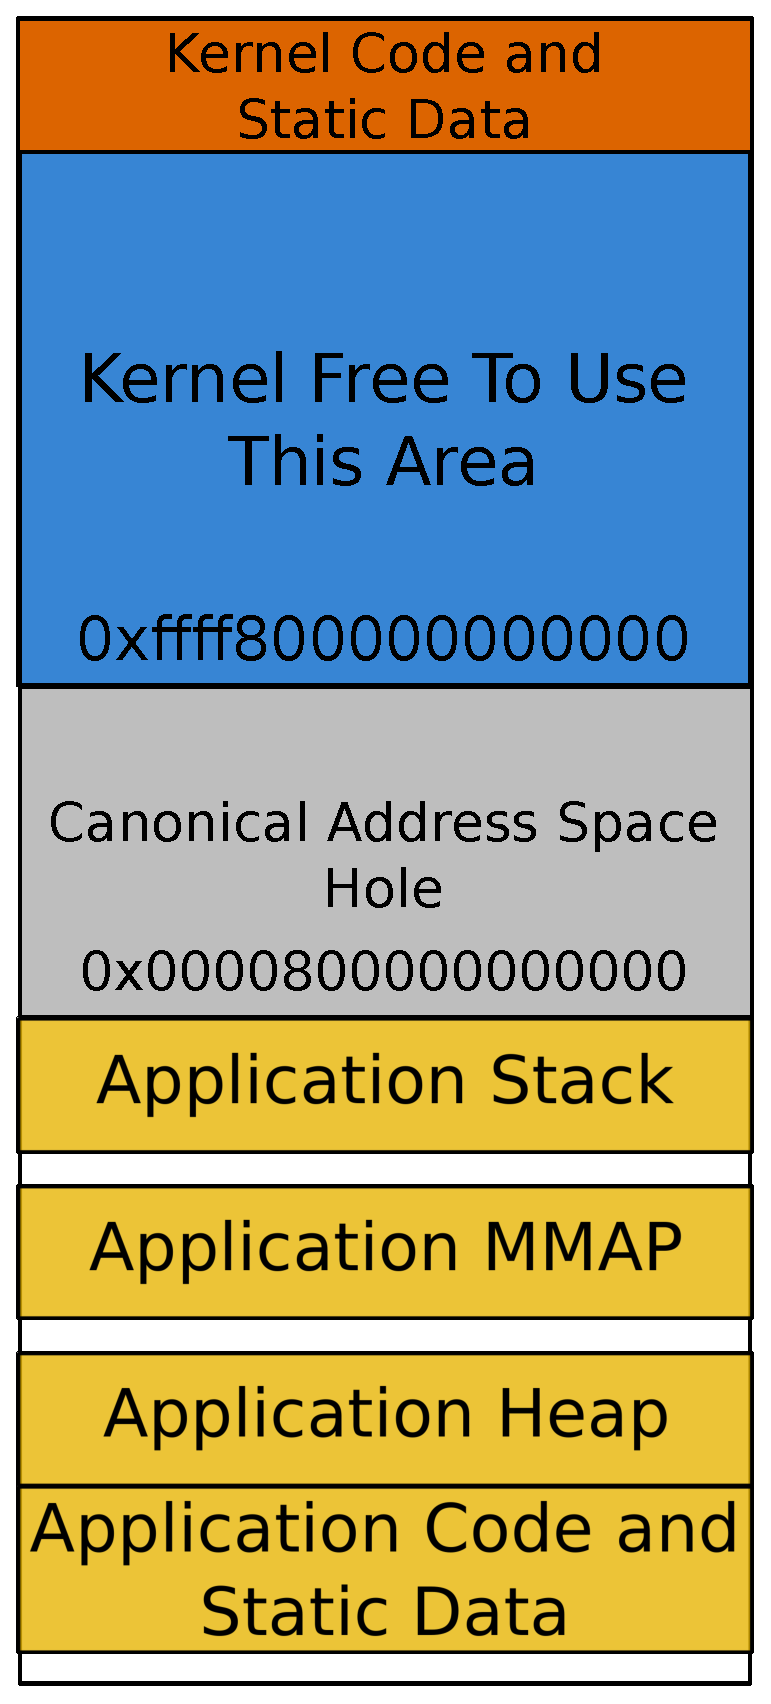
\includegraphics[width=.8\linewidth]{memmap}
  \end{column}

  \begin{column}{.6\textwidth}
    \begin{itemize}
      \item Application Stack - аллоцируется ОС при старте программы
      \item Application MMAP - разделяемые библиотеки, mmap/munmap
      \item Application Heap - malloc берет память отсюда, изменяется системным вызовом sbrk
      \item Application Code and Static Data - статическая не привелигерованная память
    \end{itemize}
  \end{column}
\end{columns}

\end{frame}


  \section{Boot Allocator}

Если вы решите использовать одну из модификация Buddy Allocator-а, то вам,
вероятно, понадобится еще один аллокатор для аллокации служебной информации,
чтобы инициализировать Buddy Allocator. Ситуация усугубляется тем, что вы к
этому моменту еще не успеете загрузить свою полноценную таблицу страниц
\footnote{Для того, чтобы ее создать, скорее всего, нужен аллокатор страниц,
которого еще нет.}.

Проблема однако решается довольно просто - вам нужен еще один, очень простой
аллокатор, который будет аллоцировать участки физической памяти из тех областей,
для которых уже есть отображение в начальной таблице страниц (на первые 4GB
физической памяти у вас отображены два участка виртуальной - вам предлагается
использовать участок сразу за "канонической дырой") используя информацию из
карты памяти.

На этот аллокатор не налагается серьезных ограничений, т. е.:

\begin{itemize}
  \item вы можете ограничить количество объектов, которые этот аллокатор может
        аллоцировать в принципе (хранить информацию о них в статическом массиве);
  \item вам не обязательно поддерживать освобождение (память нужная Buddy
        Allocator-у никогда не будет освобождена);
\end{itemize}

Однако вам необходимо проследить, чтобы аллоцированные участки памяти были
зарезервированы (так же как это должно быть сделано для памяти ядра), чтобы
никто больше не мог их использовать.

  \section{Изменения в предоставляемом коде}

В предоставленный для первого задания код были внесенные кое-какие изменения:

\begin{itemize}
  \item в kernel.ld было добавлена память под начальную таблицу страниц - если
        вы не вносили изменений kernel.ld, то конфликтов быть не должно;
  \item bootstrap.S - identity mapping и виртуальная память после "канонической
        дыры" теперь отображены на первые 4GB физической памяти;
  \item в файл memory.h были добавлены функции pa и va, которые позволяют
        получить по виртуальному адресу из участка сразу после "канонической
        дыры" физический адрес и наоборот.
\end{itemize}

Кроме того к коду был добавлен еще один заголовочный файл - paging.h. Этот файл
содержит следующие функции:

\begin{itemize}
  \item pte\_preset, pte\_user, pte\_write и pte\_large - проверяют, установлен
        ли соответствующий бит в записи таблицы страниц (бит описываются
        соответствующими define-ами);
  \item pte\_phys - достает из записи таблицы страниц физический адрес таблицы
        следующего уровня или страницы памяти, на которую отображен
        соответствующий виртуальный адрес;
  \item pml\*\_i - функции позволяющие получить индекс в таблице
        соответсвующего уровня (короче говоря, они парсят виртуальный адрес);
  \item page\_off - возвращает по виртуальному адресу смещение внутри 4KB
        страницы (оставшаяся часть парсинга виртуального адреса);
  \item canonical и linear - преобразовывают виртуальный адрес в не каноническом
        формате в канонический, и наоборот;
  \item load\_pml4 - загружается в cr3 переданный физический адрес;
  \item store\_pml4 - возвращает значение записанное в cr3;
  \item flush\_tlb\_addr - сбрасывает запись TLB соответствующую переданному
        виртуальному адресу;
  \item flush\_tlb - сбрасывает все записи в TLB (просто перезаписывает cr3
        старым значением).
\end{itemize}

  \section{Вопросы и ответы}



  \bibliography{hw2}{}
  \bibliographystyle{apalike}
\end{document}
